
\subsubsection{Дизайн пользовательского интерфейса}

На основании составленных шаблонов для интерфейса клиентской части была выполнена
их реализация и стилизация.

Для обозначения элементов интерфейса конструктора Telegram-ботов были выбраны следующие цвета:
\begin{itemize}
	\item серый;
	\item синий;
	\item зелёный;
	\item красный;
	\item желтый.
\end{itemize}

Также у каждых цветов были выбраны более светлые оттенки для обозначения фонов неактивных элементов, таких как кнопки.

Преобладающий цвет – синий, он является основным для конструктора.
Он, а также его более светлые оттенки используются
для обозначения компонентов в редакторе бота,
а также для стилизации шапки веб-приложения.
Также данный цвет служит для обозначения кнопок, которые
обеспечиваю переход на другие страницы.

Серый цвет является основным фоновым для веб-приложения,
на нём располагаются белые плитки. Плитка представляет
собой группу элементов интерфейса конструктора.

Зелёный цвет применяется для обозначения кнопок,
благодаря которым будет происходить добавление объектов
конструктора или изменение их состояния на активное.

Красный цвет служит для метки тех элементов,
которые способны удалить объекты конструктора,
или для обозначения выходов ошибок у компонентов.

Жёлтый цвет применяется для обозначения элементов интерфейса,
которые позволяют вернуться назад по страницам,
либо служат для изменения состояния
объектов конструктора на неактивное или для их индикации.

Экранные формы пользовательского интерфейса конструктора представлена
на рисунках~\ref{f:signin-page}-\ref{f:editor-page}.

{

\newcommand{\scale}{0.95}

\begin{figure}[H]
	\centering
	\vspace{\toppaddingoffigure}
	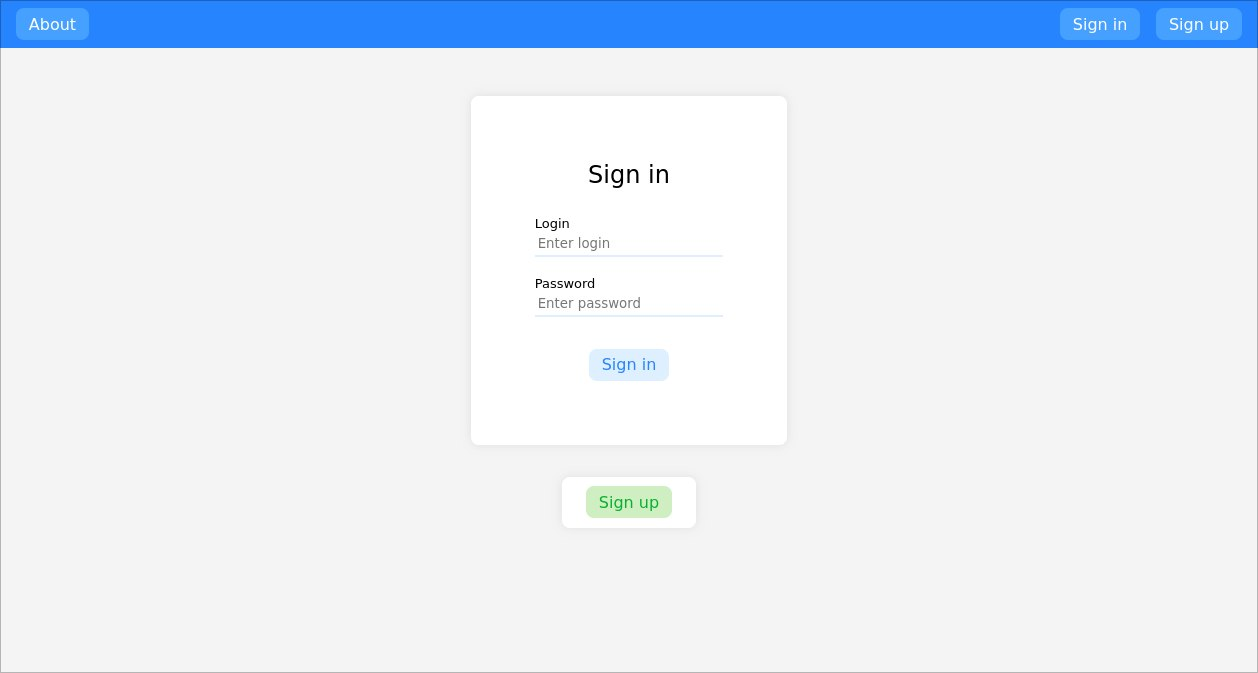
\includegraphics[width=\scale\textwidth]{/pages/signin}
	\caption{Страница входа в приложение}
	\label{f:signin-page}
\end{figure}


\begin{figure}[H]
	\centering
	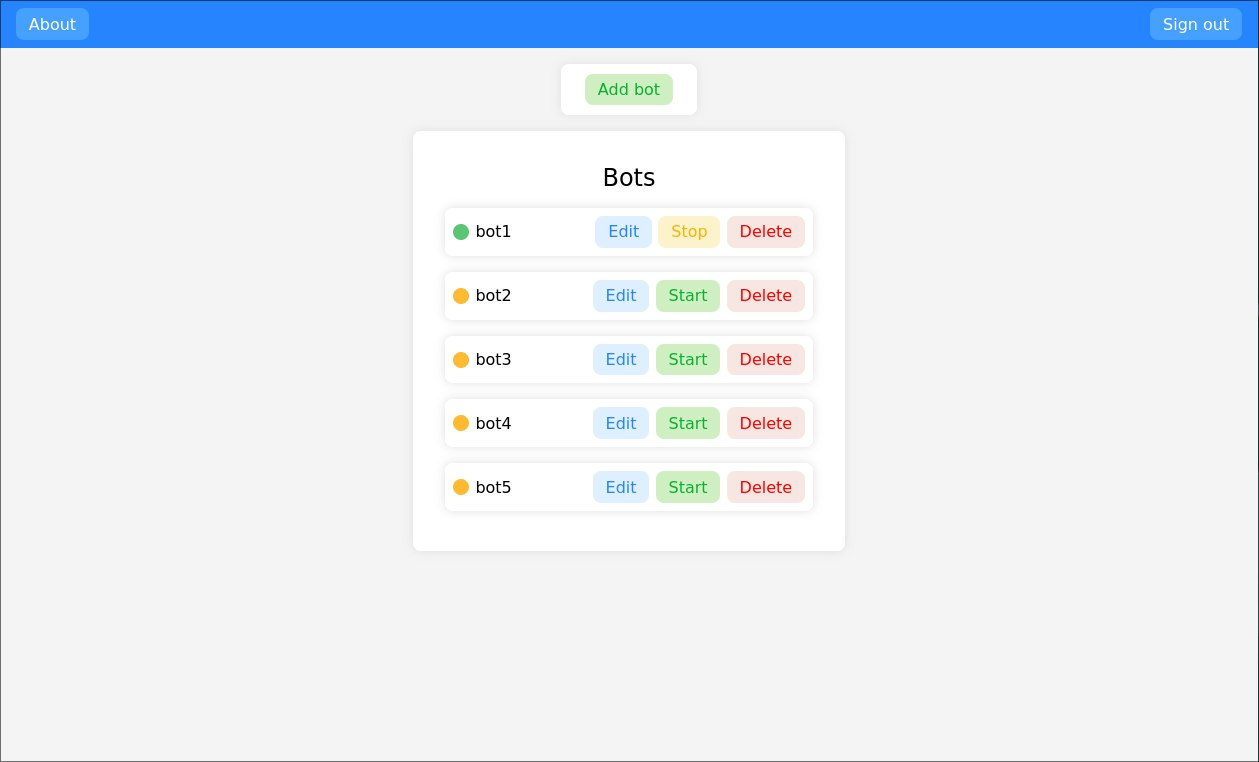
\includegraphics[width=\scale\textwidth]{/pages/bot-list}
	\caption{Страница списка ботов}
	\label{f:bot-list-page}
\end{figure}

\begin{figure}[H]
	\centering
	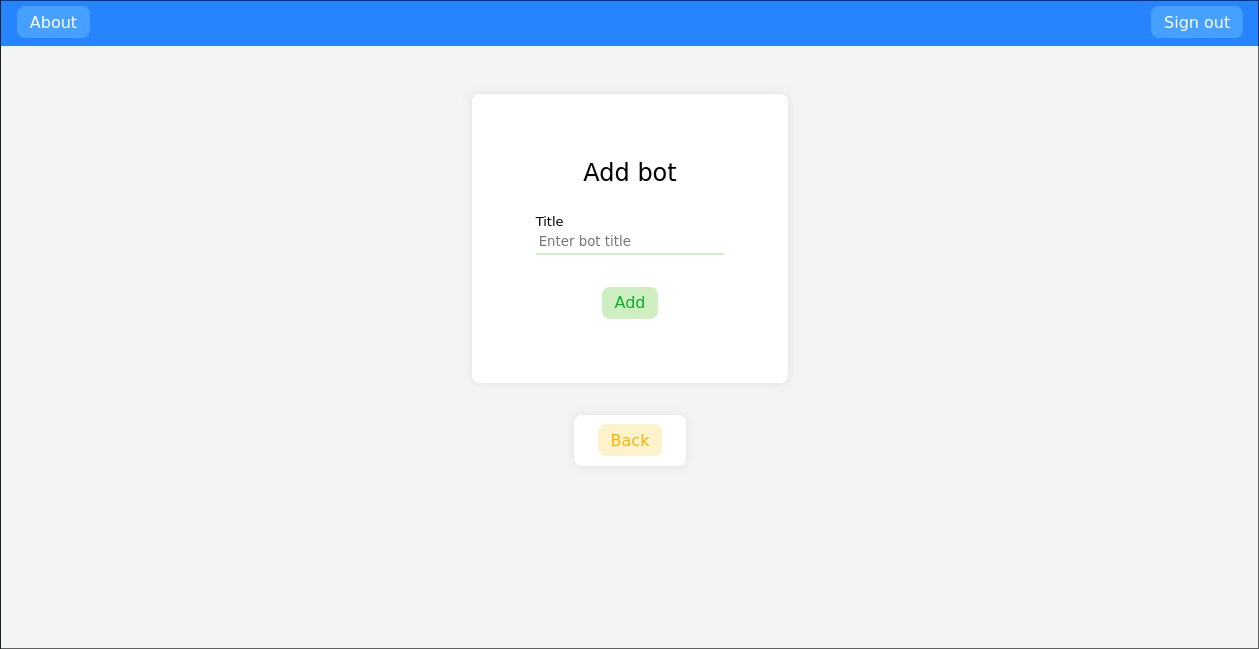
\includegraphics[width=\scale\textwidth]{/pages/add-bot}
	\caption{Страница добавления бота}
	\label{f:add-bot-page}
\end{figure}

\begin{figure}[H]
	\centering
	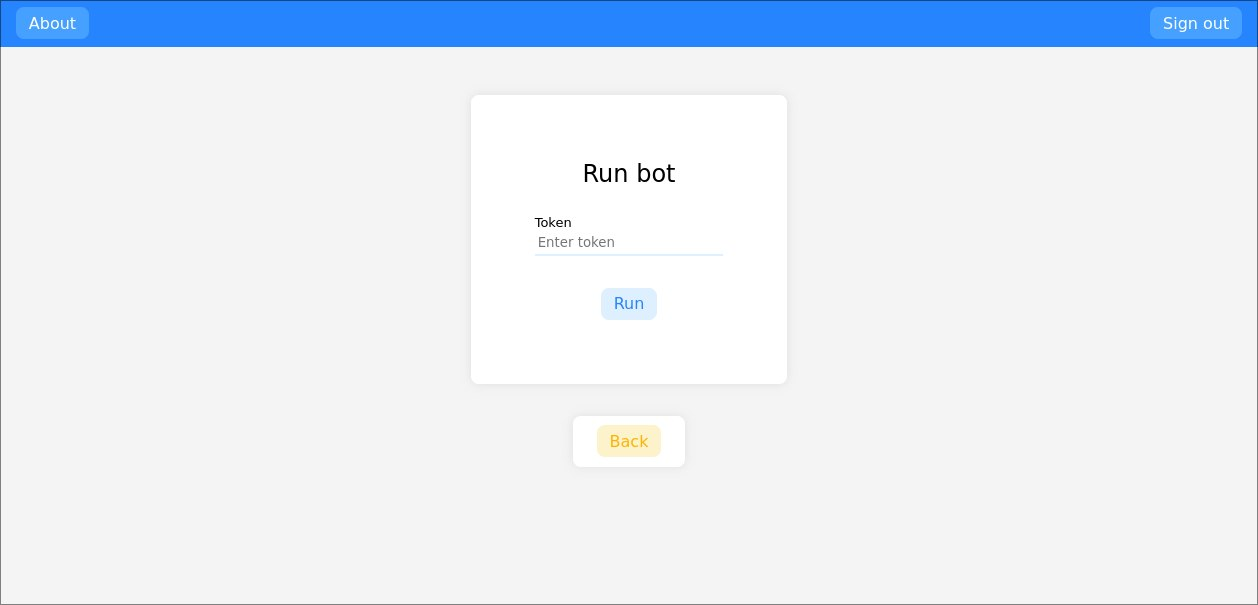
\includegraphics[width=\scale\textwidth]{/pages/run-bot}
	\caption{Страница запуска бота}
	\label{f:run-bot-page}
\end{figure}


\begin{figure}[H]
	\centering
	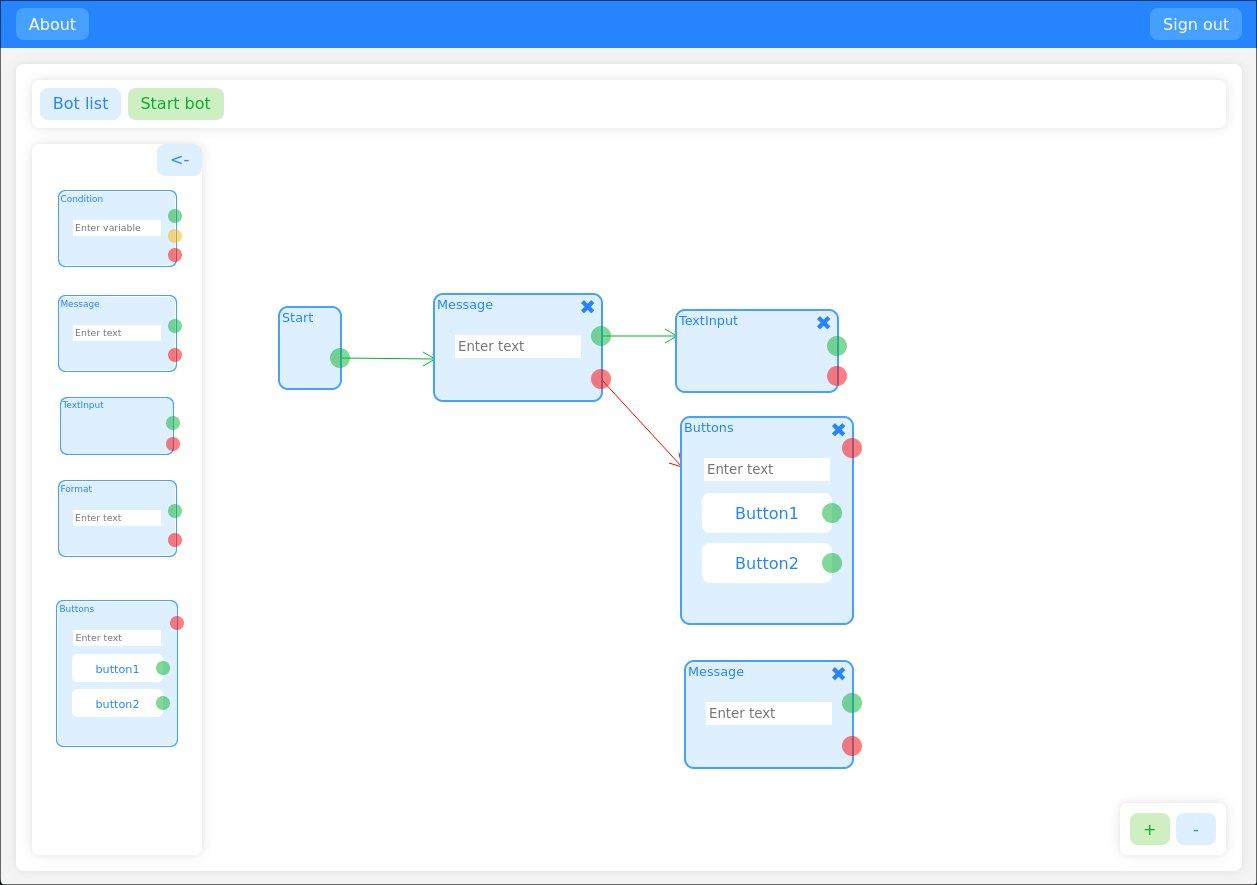
\includegraphics[width=\scale\textwidth]{/pages/editor}
	\caption{Страница визуального редактора}
	\label{f:editor-page}
\end{figure}

}
